\documentclass[conference,a4paper]{IEEEtran}
\IEEEoverridecommandlockouts
\usepackage[utf8]{inputenc}
\usepackage[T1]{fontenc}
\usepackage[spanish,es-noshorthands,es-tabla]{babel}
\usepackage{cite}
\usepackage{graphicx}
\usepackage{booktabs}
\usepackage{tikz}
\usetikzlibrary{arrows.meta,positioning}
\usepackage[hidelinks]{hyperref}
\usepackage{xurl}
\graphicspath{{figures/}{../../figuras/01_articulos_eda/}{../../figuras/02_articulos_clustering_reglas/}{../../figuras/03_imu_perfiles/}{../../figuras/04_ml_clasificacion/}{../../figuras/05_catalogo_datasets/}{../../figuras/06_regresion/}{../../figuras/07_cloud_aws/}{capturas/}}
\renewcommand{\IEEEkeywordsname}{Palabras clave}

% Inserta la captura si existe; si no, deja un recuadro con su nombre
\newcommand{\captura}[2]{\IfFileExists{capturas/#1}{\includegraphics[width=#2]{capturas/#1}}{\fbox{\parbox[c][2.2cm][c]{#2}{\centering\small Captura: \texttt{#1}}}}}

\begin{document}

\title{Detección de cojera equina mediante analítica de datos y computación en la nube: avance del proyecto integrador}

\author{\IEEEauthorblockN{Carlos Josué Barrera Vargas}
\IEEEauthorblockA{Ingeniería de Datos e Inteligencia Artificial\\
Universidad Santo Tomás, Seccional Tunja\\
Repositorio: \url{https://github.com/Cjoh210/Proyecto_Deteccion_Marcha_Equina}}}

\maketitle

\begin{abstract}
Este avance presenta la fase exploratoria de un sistema de apoyo para detectar cojera en caballos, que en su versión final analizará videos de la marcha. En esta etapa se construyó la base de conocimiento del proyecto: un corpus de artículos científicos obtenido mediante consumo de una API pública, limpiado, explorado y analizado con clustering y reglas de asociación, junto con un catálogo de datasets públicos perfilado por similitud. Los resultados muestran un área que se desplaza hacia la visión por computador, con poca investigación aplicada a caballos y casi ninguna en Colombia, y sin datasets abiertos que combinen video equino y cojera. La infraestructura en AWS se diseñó y desplegó como código con Terraform, con un costo estimado prácticamente nulo.
\end{abstract}

\begin{IEEEkeywords}
cojera equina, minería de datos, clustering, reglas de asociación, computación en la nube, Terraform
\end{IEEEkeywords}

\section{Introducción}
La cojera es uno de los problemas de salud más frecuentes y costosos en los caballos~\cite{nehs2013,usda1998}. Su diagnóstico depende principalmente de la observación del veterinario mientras el animal trota, una evaluación que resulta poco consistente cuando la cojera es leve: distintos expertos suelen llegar a conclusiones diferentes sobre el mismo caballo~\cite{keegan2010,hammarberg2016}.

Colombia tiene una población equina cercana al millón de animales~\cite{agronegocios2025}, con un peso cultural y económico importante en regiones como Boyacá. Una herramienta objetiva y de bajo costo, capaz de estimar la presencia de cojera a partir de un video tomado con el celular, sería útil para veterinarios de campo y criadores. Este documento reporta la primera fase del proyecto, orientada a comprender el estado del arte y los datos disponibles antes de construir el sistema de visión.

\section{Planteamiento del problema}
La detección temprana de la cojera es subjetiva y los métodos objetivos existentes, como sensores corporales o sistemas de captura de movimiento, son costosos y poco accesibles en el contexto rural. Surge entonces la pregunta: \emph{¿es posible estimar la presencia de cojera en caballos a partir de información de movimiento obtenida con tecnología accesible?}

\textbf{Objetivo general.} Desarrollar un sistema de apoyo a la detección de cojera equina basado en análisis de datos de la marcha y desplegado en la nube.

\textbf{Objetivos de este avance.} Construir un corpus del estado del arte mediante una fuente externa; limpiarlo, explorarlo y descubrir sus perfiles temáticos; identificar los datasets públicos útiles para el proyecto; y diseñar la infraestructura en la nube.

\textbf{Alineación con los ODS.} El proyecto se vincula con el ODS 3, Salud y bienestar, bajo el enfoque de Una Salud que integra la salud animal y humana~\cite{un2015}, y con el ODS 8, Trabajo decente y crecimiento económico, por su impacto en un sector rural que genera empleo.

\section{Estructura general del sistema}
La Fig.~\ref{fig:sistema} resume el sistema propuesto. Las fuentes de datos alimentan un repositorio central en la nube; el módulo de minería prepara y analiza los datos; y en fases posteriores un modelo de aprendizaje automático, alimentado por medidas de la marcha extraídas de video, se ofrecerá como servicio web.

\begin{figure}[t]
\centering
\begin{tikzpicture}[node distance=4mm, font=\scriptsize,
  b/.style={draw, rounded corners=2pt, align=center, minimum height=8mm, text width=15mm, fill=#1!12},
  b/.default=blue, >={Stealth[length=1.5mm]}]
\node[b=orange] (f) {Fuentes\\externas};
\node[b=green, right=of f] (s3) {Data lake\\en la nube};
\node[b, right=of s3] (m) {Minería\\de datos};
\node[b=gray, right=of m] (ml) {Modelo y\\servicio web};
\draw[->] (f) -- (s3); \draw[->] (s3) -- (m); \draw[->, dashed] (m) -- (ml);
\end{tikzpicture}
\caption{Estructura general del sistema. En gris, el componente de fases posteriores.}
\label{fig:sistema}
\end{figure}

\section{Minería de datos}
\subsection{Fuentes y adquisición}
La fuente principal es OpenAlex, un índice abierto de publicaciones científicas que se consulta mediante una API~\cite{priem2022}. Un script en Python realizó cinco búsquedas temáticas sobre cojera equina, marcha, sensores, visión por computador y detección de cojera en otras especies, y almacenó los resultados en formato tabular. Como segunda fuente se construyó un catálogo de catorce datasets públicos relacionados, con sus características principales y el enlace de origen de cada uno.

\subsection{Limpieza y tratamiento de nulos y outliers}
Se fusionaron los artículos repetidos entre búsquedas, se descartaron documentos no científicos y fuera del periodo de estudio, y se aplicó un filtro de pertinencia temática. Los valores faltantes en país y resumen se trataron como categorías o se reemplazaron por el título y las palabras clave, sin inventar información. Para los outliers se analizó el impacto de cada artículo ajustado por su antigüedad: los casos atípicos no se eliminaron, porque corresponden a los trabajos más influyentes del área, principalmente herramientas de visión por computador.

\subsection{Análisis exploratorio}
La Fig.~\ref{fig:tendencia} muestra que la producción científica crece de forma sostenida y que, en los últimos años, la visión por computador pasó a ser el enfoque dominante frente a los estudios clínicos tradicionales. La investigación se concentra en Estados Unidos, Europa y China, con una participación latinoamericana marginal.

\begin{figure}[t]
\centering
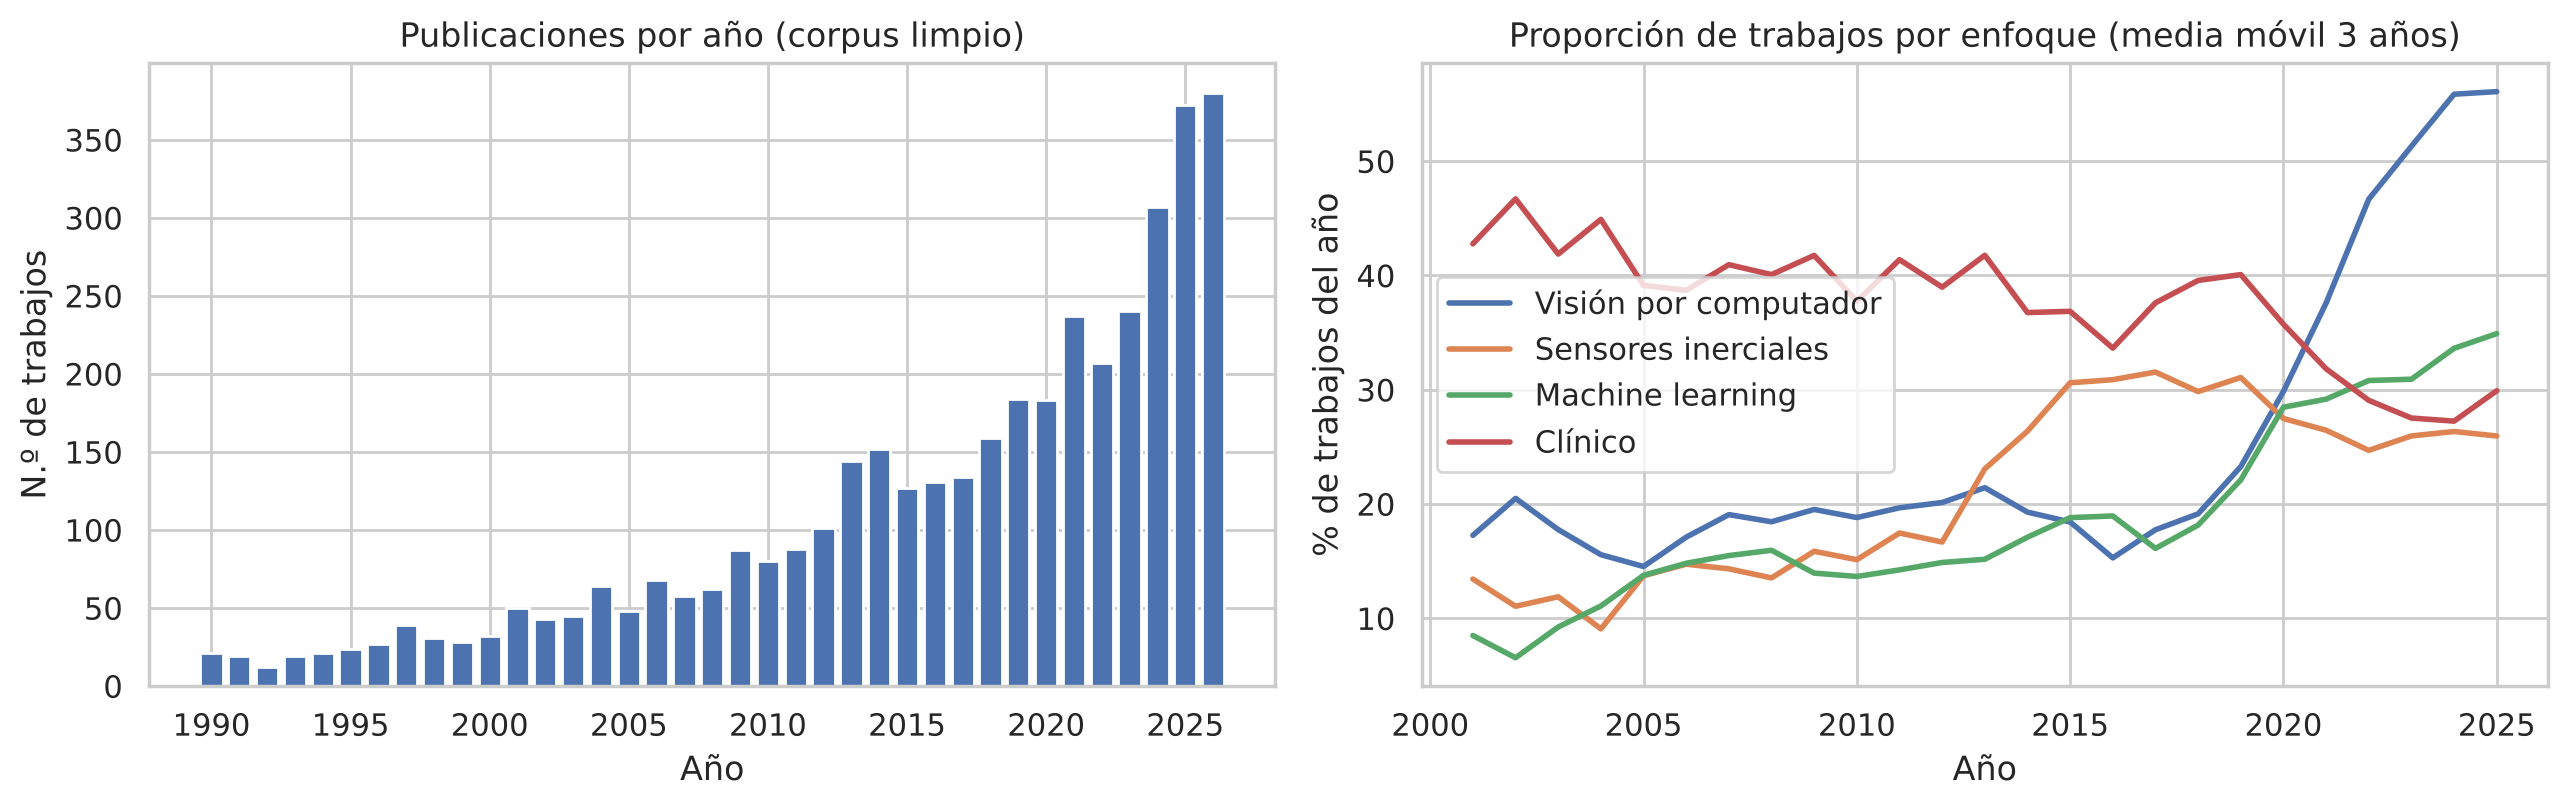
\includegraphics[width=\columnwidth]{art_tendencia_anual.png}
\caption{Publicaciones por año y proporción de trabajos según su enfoque.}
\label{fig:tendencia}
\end{figure}

\subsection{Clustering y reglas de asociación}
Los textos de los artículos se transformaron en vectores numéricos y se agruparon con K-Means. Se identificaron ocho líneas de investigación que separan un bloque clínico tradicional de un bloque tecnológico reciente, formado por estimación de pose, visión, sensores y detección en bovinos (Fig.~\ref{fig:tsne}). Las reglas de asociación entre palabras clave confirmaron que los métodos de pose animal provienen de la pose humana y que la detección automática de cojera se ha desarrollado sobre todo en vacas lecheras.

\begin{figure}[t]
\centering
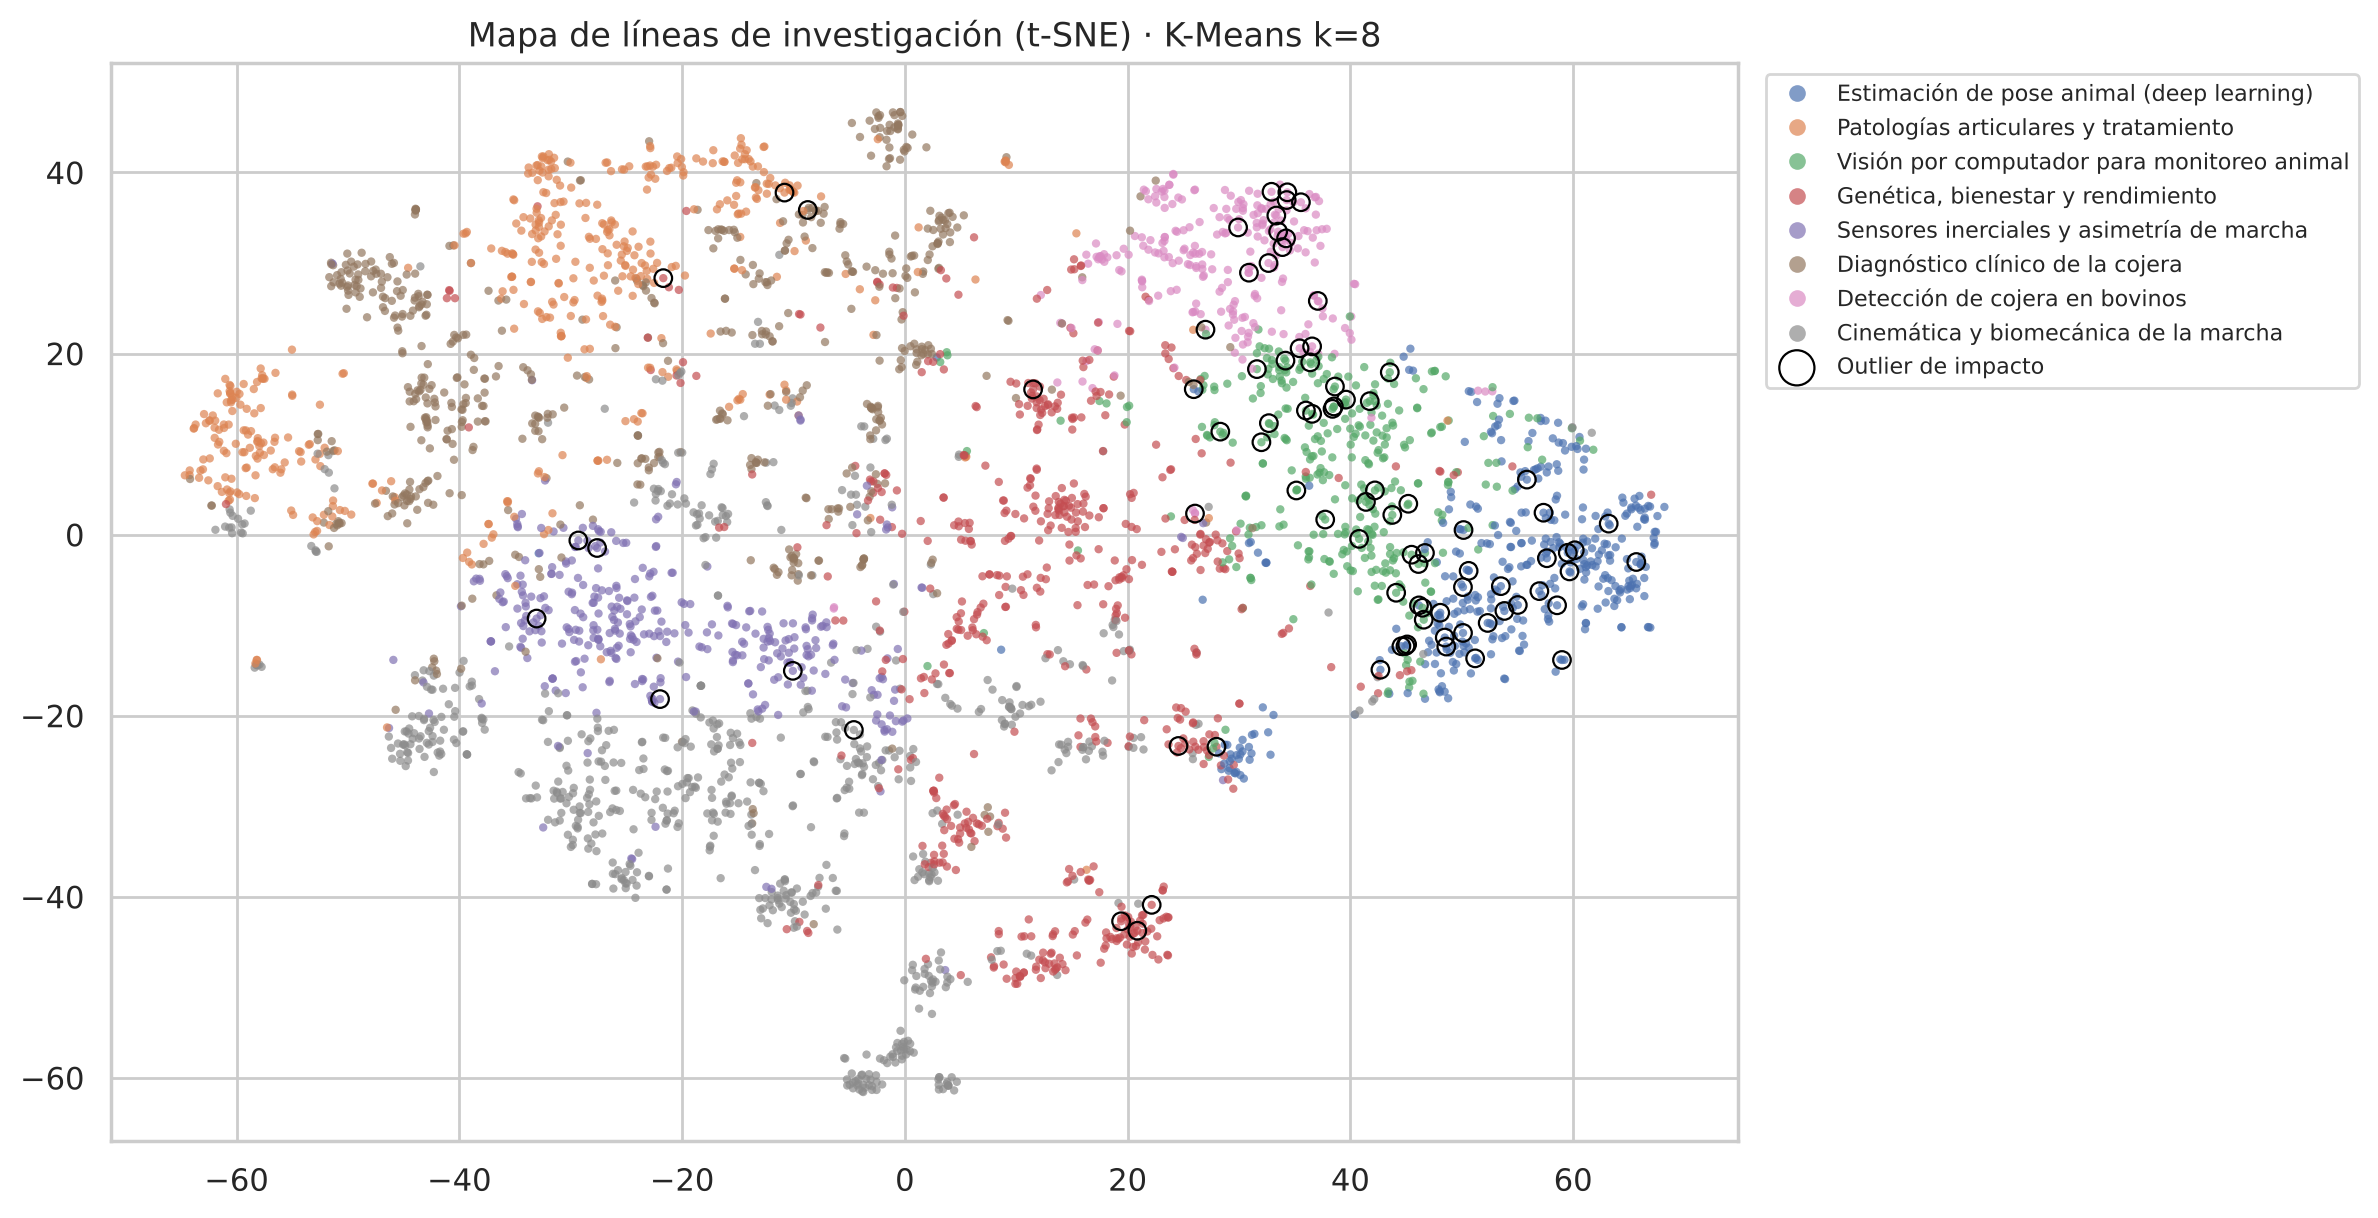
\includegraphics[width=0.95\columnwidth]{art_tsne_clusters.png}
\caption{Mapa de las líneas de investigación encontradas por clustering.}
\label{fig:tsne}
\end{figure}

\subsection{Perfilamiento de datasets}
Los catorce datasets se compararon con una medida de similitud apta para variables mixtas y se agruparon jerárquicamente. Aparecen cuatro perfiles: captura de movimiento de caballos, sensores con etiqueta de cojera, imágenes de pose y videos con puntos anatómicos. Ninguno combina video de caballos con etiqueta de cojera, lo que define la estrategia de datos de las fases siguientes (Fig.~\ref{fig:aptitud}).

\begin{figure}[t]
\centering
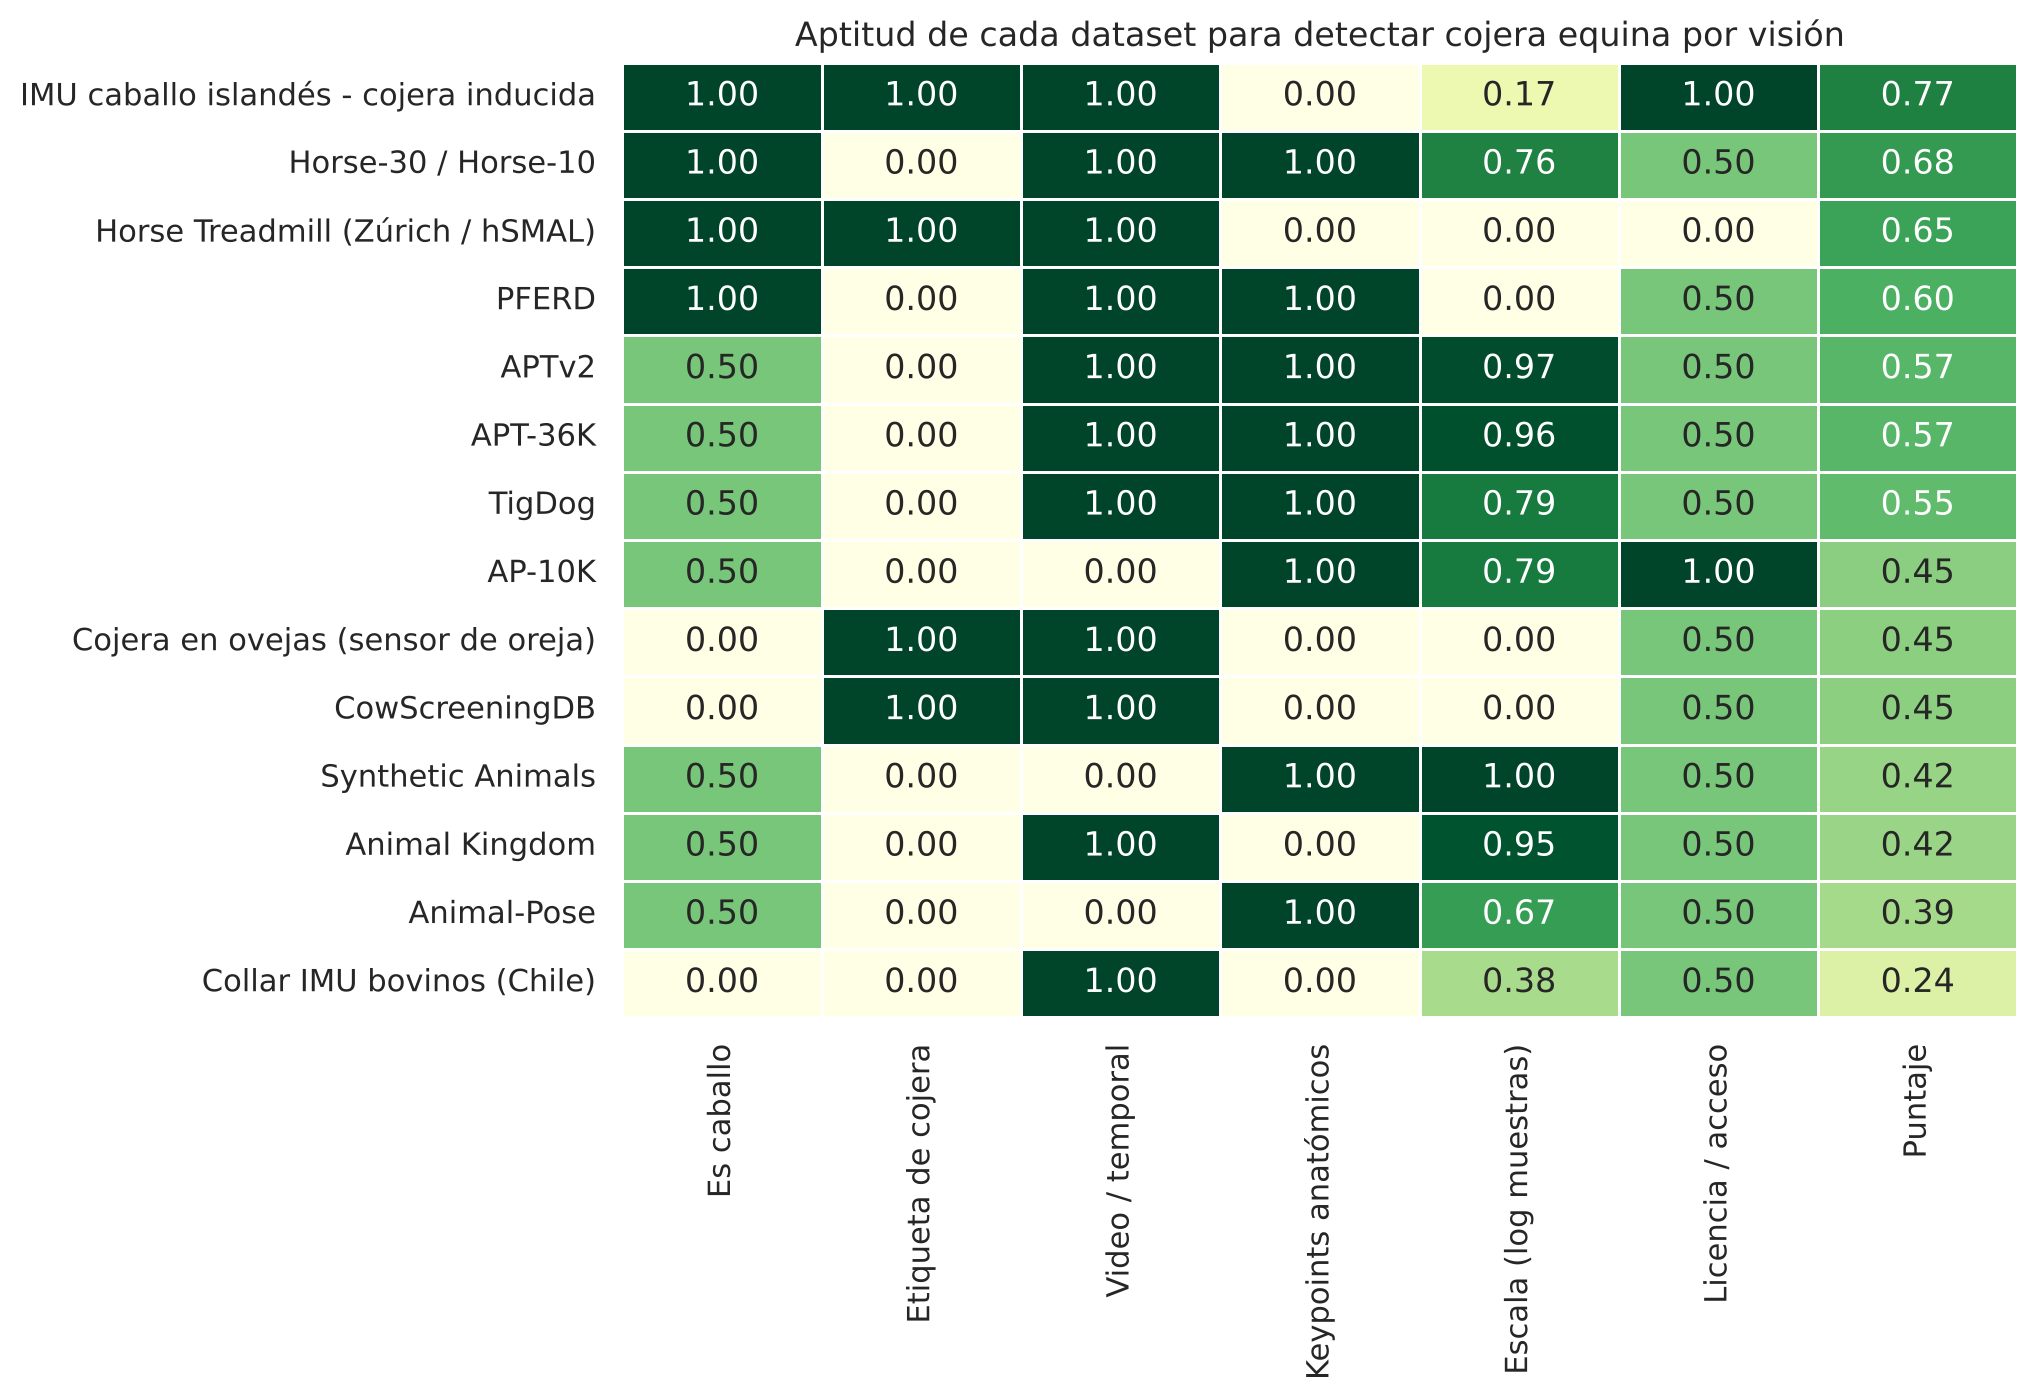
\includegraphics[width=0.9\columnwidth]{cat_matriz_aptitud.png}
\caption{Aptitud de cada dataset para el objetivo del proyecto.}
\label{fig:aptitud}
\end{figure}

\section{Infraestructura en la nube}
\subsection{Arquitectura}
Se eligió AWS con un diseño sin servidores, adecuado para una carga intermitente porque solo genera costo cuando se usa (Fig.~\ref{fig:aws}). Una función Lambda programada consulta la API cada semana y guarda los resultados en un data lake en S3; Glue y Athena permiten consultarlos con SQL; DynamoDB registrará las predicciones; y una API servirá el modelo en fases posteriores. CloudWatch y un presupuesto con alertas vigilan errores y costos.

\begin{figure}[t]
\centering
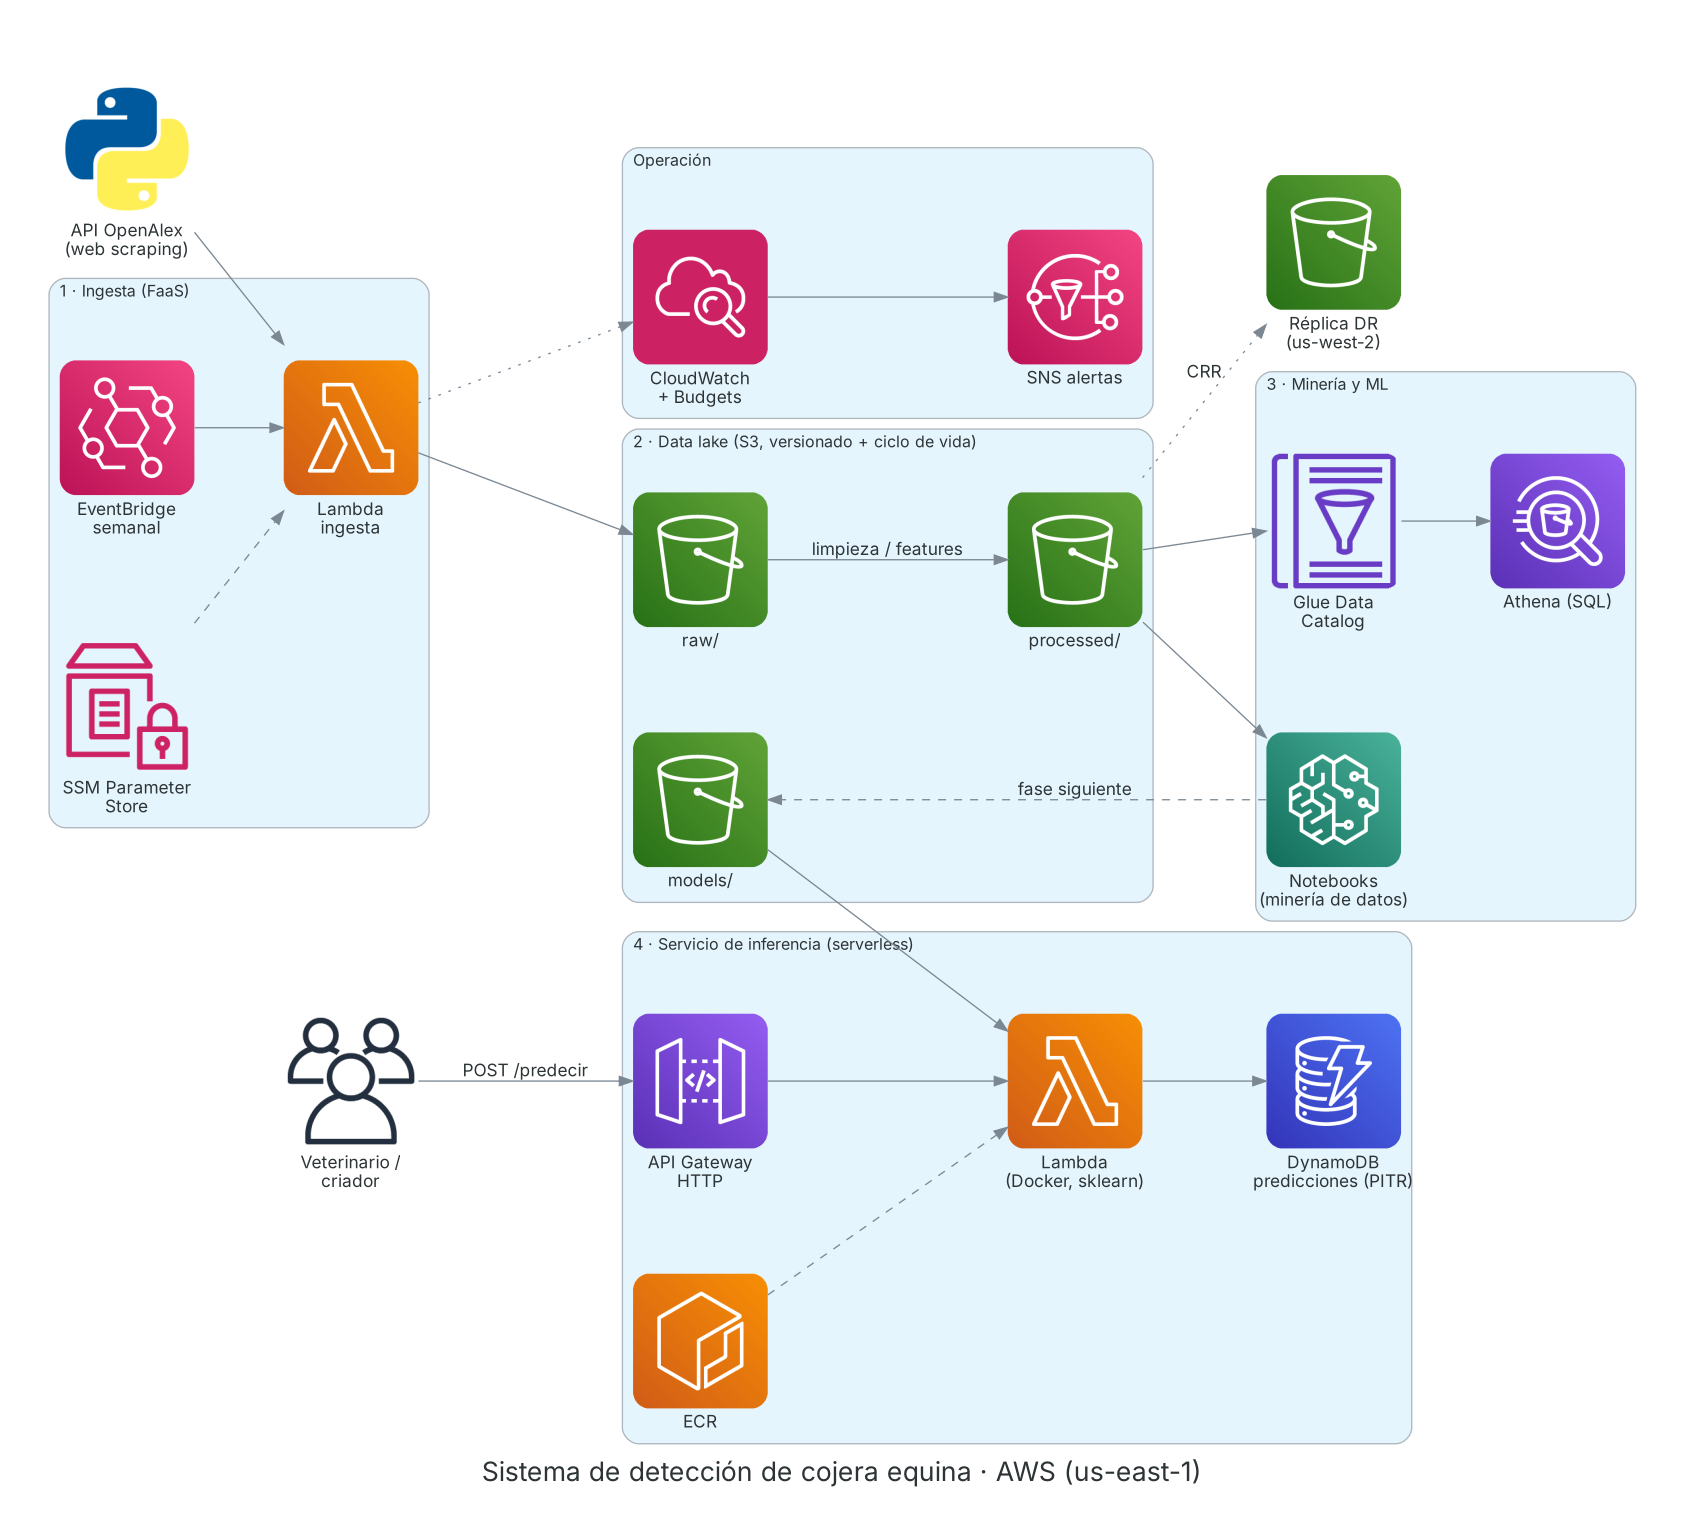
\includegraphics[width=0.8\columnwidth]{arquitectura_aws_avance.png}
\caption{Arquitectura propuesta en AWS.}
\label{fig:aws}
\end{figure}

\subsection{Infraestructura como código}
Toda la infraestructura se definió en Terraform y se desplegó en una cuenta de AWS (Fig.~\ref{fig:apply}). La función de ingesta se ejecutó en la nube y almacenó en S3 el mismo corpus obtenido en el análisis local (Fig.~\ref{fig:s3}), lo que confirma que el proceso es reproducible.

\begin{figure}[t]
\centering
\captura{terraform_apply.png}{\columnwidth}
\caption{Despliegue de la infraestructura con Terraform.}
\label{fig:apply}
\end{figure}

\begin{figure}[t]
\centering
\captura{s3_openalex.png}{\columnwidth}\\[2mm]
\captura{lambda_ingesta.png}{\columnwidth}
\caption{Corpus almacenado en S3 por la función Lambda de ingesta.}
\label{fig:s3}
\end{figure}

\subsection{Estimación preliminar de costos}
Con precios de lista en la región us-east-1, el escenario académico cuesta menos de medio dólar al mes y queda cubierto casi por completo por la capa gratuita. Una proyección con cincuenta clínicas usando el sistema se mantiene por debajo de quince dólares mensuales, con el almacenamiento como principal rubro.

\section{Trabajo siguiente}
La próxima fase incorporará datos de sensores de caballos con cojera para identificar qué medidas de la marcha la delatan, entrenará un modelo de clasificación y activará la API de inferencia. Posteriormente, la visión por computador estimará esas mismas medidas a partir de video.

\begin{thebibliography}{9}
\bibitem{nehs2013} ``Equine health survey highlights the prevalence of lameness,'' \emph{Veterinary Record}, vol.~173, no.~6, p.~132, 2013.
\bibitem{usda1998} USDA APHIS, ``National economic cost of equine lameness, colic, and equine protozoal myeloencephalitis in the United States,'' NAHMS Equine'98.
\bibitem{keegan2010} K.~G. Keegan \emph{et al.}, ``Repeatability of subjective evaluation of lameness in horses,'' \emph{Equine Vet. J.}, vol.~42, no.~2, pp.~92--97, 2010.
\bibitem{hammarberg2016} M.~Hammarberg, A.~Egenvall, T.~Pfau y M.~Rhodin, ``Rater agreement of visual lameness assessment in horses during lungeing,'' \emph{Equine Vet. J.}, vol.~48, no.~1, pp.~78--82, 2016.
\bibitem{agronegocios2025} Agronegocios, ``¿Cuántos caballos hay en Colombia y de esta cifra cuántos están registrados?,'' 2025.
\bibitem{un2015} Naciones Unidas, ``Transformar nuestro mundo: la Agenda 2030 para el Desarrollo Sostenible,'' A/RES/70/1, 2015.
\bibitem{priem2022} J.~Priem, H.~Piwowar y R.~Orr, ``OpenAlex: A fully-open index of scholarly works, authors, venues, institutions, and concepts,'' arXiv:2205.01833, 2022.
\end{thebibliography}

\end{document}
